% flashcards-title: Equal sharing and equal grouping
% flashcards-desc: One panel shares twelve counters among three outlined boxes. A second panel outlines four groups of three counters.
\documentclass[dvisvgm,tikz,border=8pt]{standalone}
\usetikzlibrary{arrows.meta,patterns}

\definecolor{qraNavy}{HTML}{17324D}
\definecolor{qraBlue}{HTML}{2B6CB0}
\definecolor{qraGold}{HTML}{B7791F}
\definecolor{qraPale}{HTML}{EAF2F8}
\definecolor{qraGray}{HTML}{5C6773}

\tikzset{
  qra axis/.style={draw=qraNavy, line width=1.2pt},
  qra tick/.style={draw=qraNavy, line width=1pt},
  qra guide/.style={draw=qraGray, densely dashed, line width=0.8pt},
  qra counter/.style={circle, draw=qraNavy, fill=qraPale, line width=0.9pt, minimum size=7mm, inner sep=0pt},
  qra label/.style={font=\sffamily\bfseries, text=qraNavy},
  qra small label/.style={font=\sffamily, text=qraNavy},
}

\begin{document}
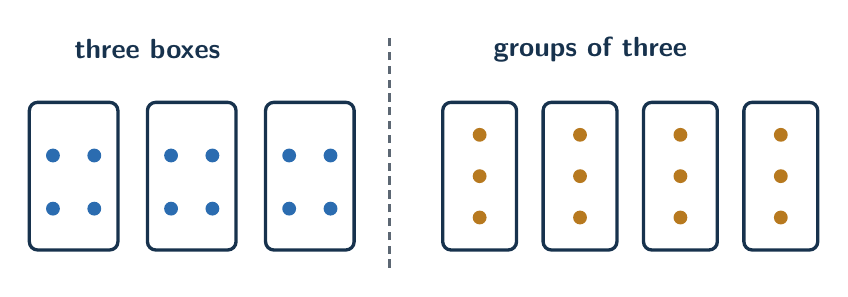
\begin{tikzpicture}[x=.75cm,y=.75cm]
  \node[qra label] at (2,2.9) {three boxes};
  \foreach \b in {0,1,2}{\draw[qra axis,rounded corners=3pt] (\b*2,-.5) rectangle +(1.5,2.5);\foreach \y in {0,1}{\foreach \x in {0,1}{\fill[qraBlue] (\b*2+.4+.7*\x,.2+.9*\y) circle (2.5pt);}}}
  \draw[qra guide] (6.1,-.8)--(6.1,3.1);
  \node[qra label] at (9.5,2.9) {groups of three};
  \foreach \b in {0,1,2,3}{\draw[qra axis,rounded corners=3pt] (7+\b*1.7,-.5) rectangle +(1.25,2.5);\foreach \y in {0,1,2}{\fill[qraGold] (7.625+\b*1.7,.05+.7*\y) circle (2.5pt);}}
\end{tikzpicture}
\end{document}
